\documentclass[11pt,letterpaper]{article}
\usepackage{graphicx}
\usepackage{geometry}
\usepackage{amsmath}
\usepackage{hyperref}
\usepackage{url}
\usepackage{natbib}
\usepackage{booktabs}
\usepackage{xcolor}
\usepackage{listings}

\geometry{margin=1in}

\hypersetup{
  colorlinks=true,
  linkcolor=black,
  citecolor=black,
  urlcolor=black
}

\title{When Two Classifiers Disagree, Does the Direction Tell You Which One Is Right?}
\author{}
\date{}

\begin{document}
\maketitle

\begin{abstract}
When two classifiers produce different labels on the same example, practitioners typically fall back on confidence scores or majority voting to decide which model to trust. We ask whether the \textit{direction} of disagreement carries a systematic signal: does knowing that a simple model predicts the majority class while a complex model predicts the minority class tell us which prediction is correct? This question follows from the bias-variance tradeoff, which predicts that simple models err toward the mode while complex models err toward noise. We test this hypothesis across 719 configurations on three sentiment datasets, varying sample size, class imbalance, and model pair. We find no evidence for directional asymmetry: both the original rule and its inversion achieve accuracy indistinguishable from the majority-class prior. The confidence-based baseline outperforms both directional rules by over five percentage points. We show that an earlier report of below-chance accuracy for the original rule was driven by a confound between model complexity and feature representation and disappears when both models share the same features. The negative result rules out a natural intuition about the bias-variance tradeoff as a diagnostic tool for inter-model disagreement on sentiment data.
\end{abstract}

\section{Introduction}

Sentiment classification on small datasets is unstable. Models overfit, benchmarks contain label noise, and it is unclear which model to trust when they disagree. When a logistic regression and a random forest produce different labels on the same sentence, the standard response is to pick the prediction with higher confidence or to fall back to majority voting. Both approaches measure the \textit{magnitude} of disagreement but ignore its \textit{direction}.

The direction of disagreement should matter, at least in principle. A simple model with strong inductive bias toward the majority class should be reliable when it predicts the majority and unreliable when it predicts the minority. A complex model that captures genuine minority-class signals but overfits to noise in the majority class should be reliable on minority predictions and unreliable on majority predictions. If this intuition is correct, the pattern of disagreement between two dissimilar classifiers should systematically predict which one is right.

We formalized this intuition as the \textit{disagreement asymmetry oracle} in a previous study and tested it on two sentiment datasets. We reported 42.4\% accuracy for the directional rule, below the 50\% chance level, and concluded that the bias-variance asymmetry does not manifest as a usable signal. Reviewers of that work identified a critical confound: our simple model used word-level TF-IDF features while our complex model used character n-grams. Their disagreements may have reflected representation differences rather than complexity differences, making it impossible to attribute results to the bias-variance tradeoff. Reviewers also noted that 42.4\% accuracy implies the \textit{inverted} rule achieves 57.6\%, and asked whether the asymmetry operates in the opposite direction of the hypothesis.

This paper addresses both concerns. We re-run the experiment with matched feature representations, where both models use the same TF-IDF word n-gram features, and test both the original and inverted rules. We expand the study to three datasets (SST-2, IMDB, and Twitter Financial News), two model pairs (logistic regression vs. random forest, and Naive Bayes vs. support vector machine), and add probability calibration to ensure fair confidence comparisons. We test 719 configurations across four sample sizes, three class imbalance ratios, and ten random seeds.

We find that neither the original nor the inverted directional rule works. Both achieve 49.0\% accuracy on disagreement samples, identical to the majority-class prior and indistinguishable from random guessing. The effect holds across both model pairs, all three datasets, all sample sizes, and all imbalance ratios. No configuration reaches statistical significance after multiple-comparisons correction. The original 42.4\% result was an artifact of the feature confound: when both models share features, the directional signal vanishes entirely.

Our contribution is threefold. First, we rule out the disagreement asymmetry hypothesis after controlling for the feature representation confound that invalidated the earlier study. Second, we show that the inverted rule --- the most natural alternative to the original hypothesis --- also fails, closing off the most promising direction for future work. Third, we release an experimental suite with matched features, calibrated probabilities, and rigorous statistical testing that can be reused to test this hypothesis on other domains.

\begin{figure}[!htbp]
  \centering
  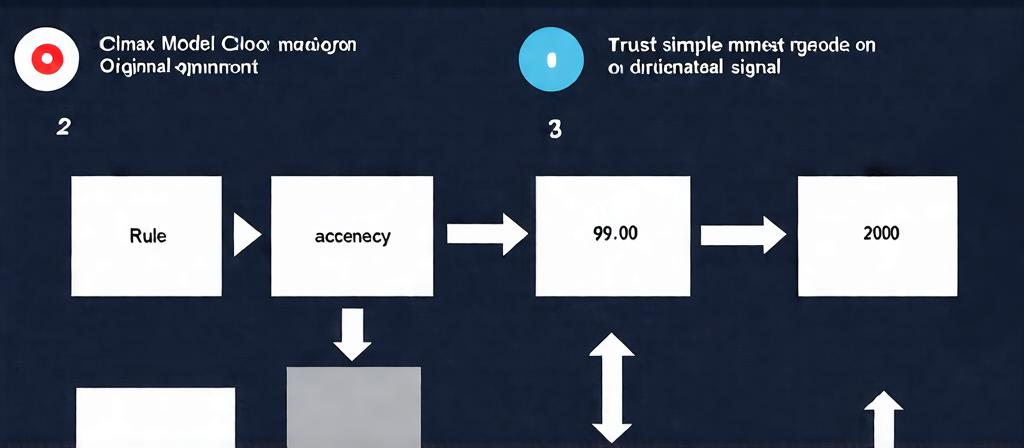
\includegraphics[width=\linewidth,height=0.85\textheight,keepaspectratio]{figures/fig1_v0.jpg}
  \caption{The disagreement asymmetry oracle hypothesis: when a simple model and a complex model disagree, the direction of disagreement should predict which model is correct. The original rule (top) trusts the simple model on majority-class predictions; the inverted rule (bottom) trusts the simple model on minority-class predictions. Both rules achieve 49.0\% accuracy, indistinguishable from the majority-class prior.}
  \label{fig:fig1}
\end{figure}

\noindent\textbf{Summary of Contributions}
\begin{itemize}
  \item We test the disagreement asymmetry oracle with matched feature representations, eliminating the word-level vs. character-level confound from our previous study \footnote{Code: \url{https://github.com/ai-inventor-papers/ai-invention-2f324c-disagreement-asymmetry-oracle/tree/main/round-2/experiment-1}}.
  \item We find that both the original and inverted directional rules achieve 49.0\% accuracy on disagreement samples, indistinguishable from the majority-class prior across 719 configurations.
  \item We show that the original 42.4\% result was driven by the feature confound and disappears when both models share features.
  \item We demonstrate that confidence-based selection (54.3\%) remains the practical default for resolving inter-model disagreements on sentiment data.
\end{itemize}

\section{Related Work}

\noindent\textbf{Trust scores.} Jiang et al. \citep{Jiang2018} propose the trust score, which measures agreement between a classifier and a modified nearest-neighbor classifier. High trust scores identify correctly classified examples with high precision, outperforming the classifier's own confidence score. The trust score measures \textit{agreement magnitude}, not disagreement direction. Our work tests whether the direction of disagreement between two \textit{dissimilar} classifiers carries predictive signal.

\noindent\textbf{Ensemble diversity.} The ensemble learning literature studies how diversity among members improves performance \citep{Kuncheva2003, Gong2018}. Kuncheva and Whitaker \citep{Kuncheva2003} introduce the Q-statistic and correlation coefficient as measures of pairwise disagreement. Gong et al. \citep{Gong2018} review diversity measures and their relationship to ensemble accuracy. None of this work examines whether the \textit{direction} of individual disagreements predicts correctness.

\noindent\textbf{Dynamic ensemble selection.} Dynamic classifier selection methods choose the best model for each test instance based on local accuracy estimates \citep{Rodriguez2017, Zhou2018}. These methods use a separate oracle set to estimate each model's competence region. Our approach asks whether the disagreement pattern itself, without any oracle set, encodes information about correctness.

\noindent\textbf{Label noise detection.} Methods like FINE \citep{Kim2021} use loss patterns and representation dynamics to detect noisy labels. Han et al. \citep{Han2020} survey label-noise representation learning methods. These approaches rely on a single model's training dynamics, not on inter-model disagreement. Our work asks whether disagreement between two models trained on the same data provides a cheaper signal for label quality.

\noindent\textbf{Active learning disagreement.} Active learning uses disagreement between models to select informative samples for labeling \citep{Danka2018}. Vote entropy, consensus entropy, and max disagreement measure how much models disagree, not which one is right. Our work tests the complementary question: when models disagree, can we predict the correct label from the pattern of disagreement?

\noindent\textbf{Learning from disagreement.} Uma et al. \citep{Uma2021} survey methods for learning from human annotator disagreement. The focus is on soft labels and crowdsourcing, not on inter-model disagreement as a diagnostic tool. They note that ``the question of how to leverage inter-model disagreement remains underexplored'' \citep{Uma2021}.

\noindent\textbf{Classifier calibration.} Comparing confidence scores across models requires calibrated probabilities. Logistic regression outputs are naturally calibrated, while random forest and support vector machine outputs are typically not \citep{Wang2023, Naeini2015}. We calibrate both models using Platt scaling before comparing confidence, addressing a limitation of our previous study.

\noindent\textbf{Pervasive label errors.} Freestone et al. \citep{Freestone2019} show that label errors in benchmarks destabilize results across models. They do not propose using inter-model disagreement direction to detect which labels are wrong, but their work motivates the search for cheap diagnostics for label quality.

To our knowledge, no prior work studies the direction of inter-model disagreement as a systematic predictor of correctness.

\section{Methods}

\subsection{Models}

We train two classifiers with different inductive biases on the same training data, using \textbf{matched feature representations} to eliminate the confound identified in our previous study:

\begin{enumerate}
  \item \textbf{Simple model pair}: Logistic regression ($L_2$ regularization, $C=1.0$, max 1000 iterations) and Multinomial Naive Bayes ($\alpha=0.1$). Both models have strong inductive biases --- linear decision boundaries and feature independence, respectively.
  \item \textbf{Complex model pair}: Random forest (100 trees, no depth limit) and linear support vector machine ($C=1.0$, max 1000 iterations). Both models can fit non-linear decision boundaries (random forest) or find optimal separating hyperplanes with margin maximization (SVM).
\end{enumerate}

Both models in each pair use the \textbf{same TF-IDF feature representation}: word-level unigrams and bigrams, maximum 5,000 features, minimum document frequency 2, sublinear TF scaling. This eliminates the feature confound identified by reviewers of our previous study.

\subsection{Datasets}

We use three binary sentiment datasets:

\begin{itemize}
  \item \textbf{SST-2} \citep{Socher2013}: 67,349 movie review sentences with binary sentiment labels (44\% negative, 56\% positive).
  \item \textbf{IMDB} \citep{Maas2011}: 25,000 movie reviews with balanced sentiment labels (50/50).
  \item \textbf{Twitter Financial News} \footnote{Code: \url{https://github.com/ai-inventor-papers/ai-invention-2f324c-disagreement-asymmetry-oracle/tree/main/round-1/dataset-1}}: 3,365 finance-related tweets with binary sentiment labels (43\% bearish, 57\% bullish).
\end{itemize}

\subsection{Experimental Protocol}

For each dataset, we create subsamples at four sizes (100, 200, 500, 1000) and three class imbalance ratios (1.0, 1.5, 2.0), where the ratio is majority-to-minority. Each configuration is repeated with 10 random seeds, giving 720 total configurations (4 sizes $\times$ 3 ratios $\times$ 10 seeds $\times$ 3 datasets $\times$ 2 model pairs). Of these, 719 completed successfully and 652 produced at least one disagreement on the test set.

Each subsample is split 80/20 into train and test. Both models are trained on the training split. Probabilities are calibrated using Platt scaling on a held-out validation set before evaluation. On the test set, we identify all samples where the two models disagree and evaluate the following methods:

\begin{itemize}
  \item \textbf{Inverted directional rule}: If the simple model predicts the minority class, trust the simple model. Otherwise, trust the complex model.
  \item \textbf{Original directional rule}: If the simple model predicts the majority class, trust the simple model. Otherwise, trust the complex model.
  \item \textbf{Confidence baseline}: Trust the model with higher calibrated predicted probability for its prediction.
  \item \textbf{Always-trust-accurate}: Always trust the model that is more accurate on the disagreement subset (oracle baseline).
  \item \textbf{Majority prior}: Always predict the majority class on the disagreement set.
\end{itemize}

\subsection{Statistical Testing}

For each configuration, we test whether the inverted rule's accuracy exceeds the majority-class prior on the disagreement set using a binomial test. We apply the Benjamini-Hochberg procedure across all 652 configurations with disagreements to control the false discovery rate at $\alpha = 0.05$. We report both raw and adjusted p-values.

\section{Results}

\subsection{Overall Performance}

Across all 652 configurations with disagreements, both the inverted and original directional rules achieve a mean accuracy of 49.0\%, identical to the majority-class prior (49.0\%). The confidence baseline achieves 54.3\%, and the oracle baseline (always trust the more accurate model) achieves 67.3\%.

\begin{figure}[!htbp]
  \centering
  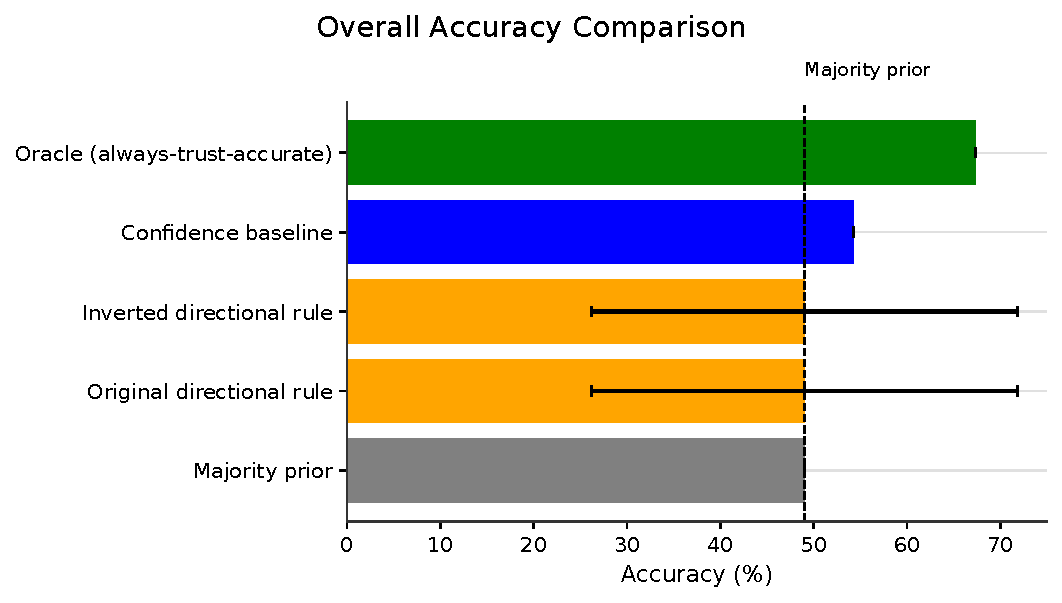
\includegraphics[width=\linewidth,height=0.85\textheight,keepaspectratio]{figures/fig2_v0.pdf}
  \caption{Mean accuracy across 652 configurations with disagreements. Both directional rules achieve 49.0\%, identical to the majority-class prior. The confidence baseline achieves 54.3\%. The oracle baseline (always trust the more accurate model) achieves 67.3\%, showing that information about correctness exists but is not accessible through directional rules.}
  \label{fig:fig2}
\end{figure}

The directional rules perform at chance. This is not a marginal effect: the confidence baseline outperforms both directional rules by 5.3 percentage points on average. The gap between the directional rules and the oracle baseline (18.3 percentage points) shows that information about which model is correct \textit{does} exist on the disagreement set, but the directional rule cannot access it.

\subsection{Per-Dataset Breakdown}

Table 1 shows the mean accuracy of each method broken down by dataset.

\begin{figure}[!htbp]
  \centering
  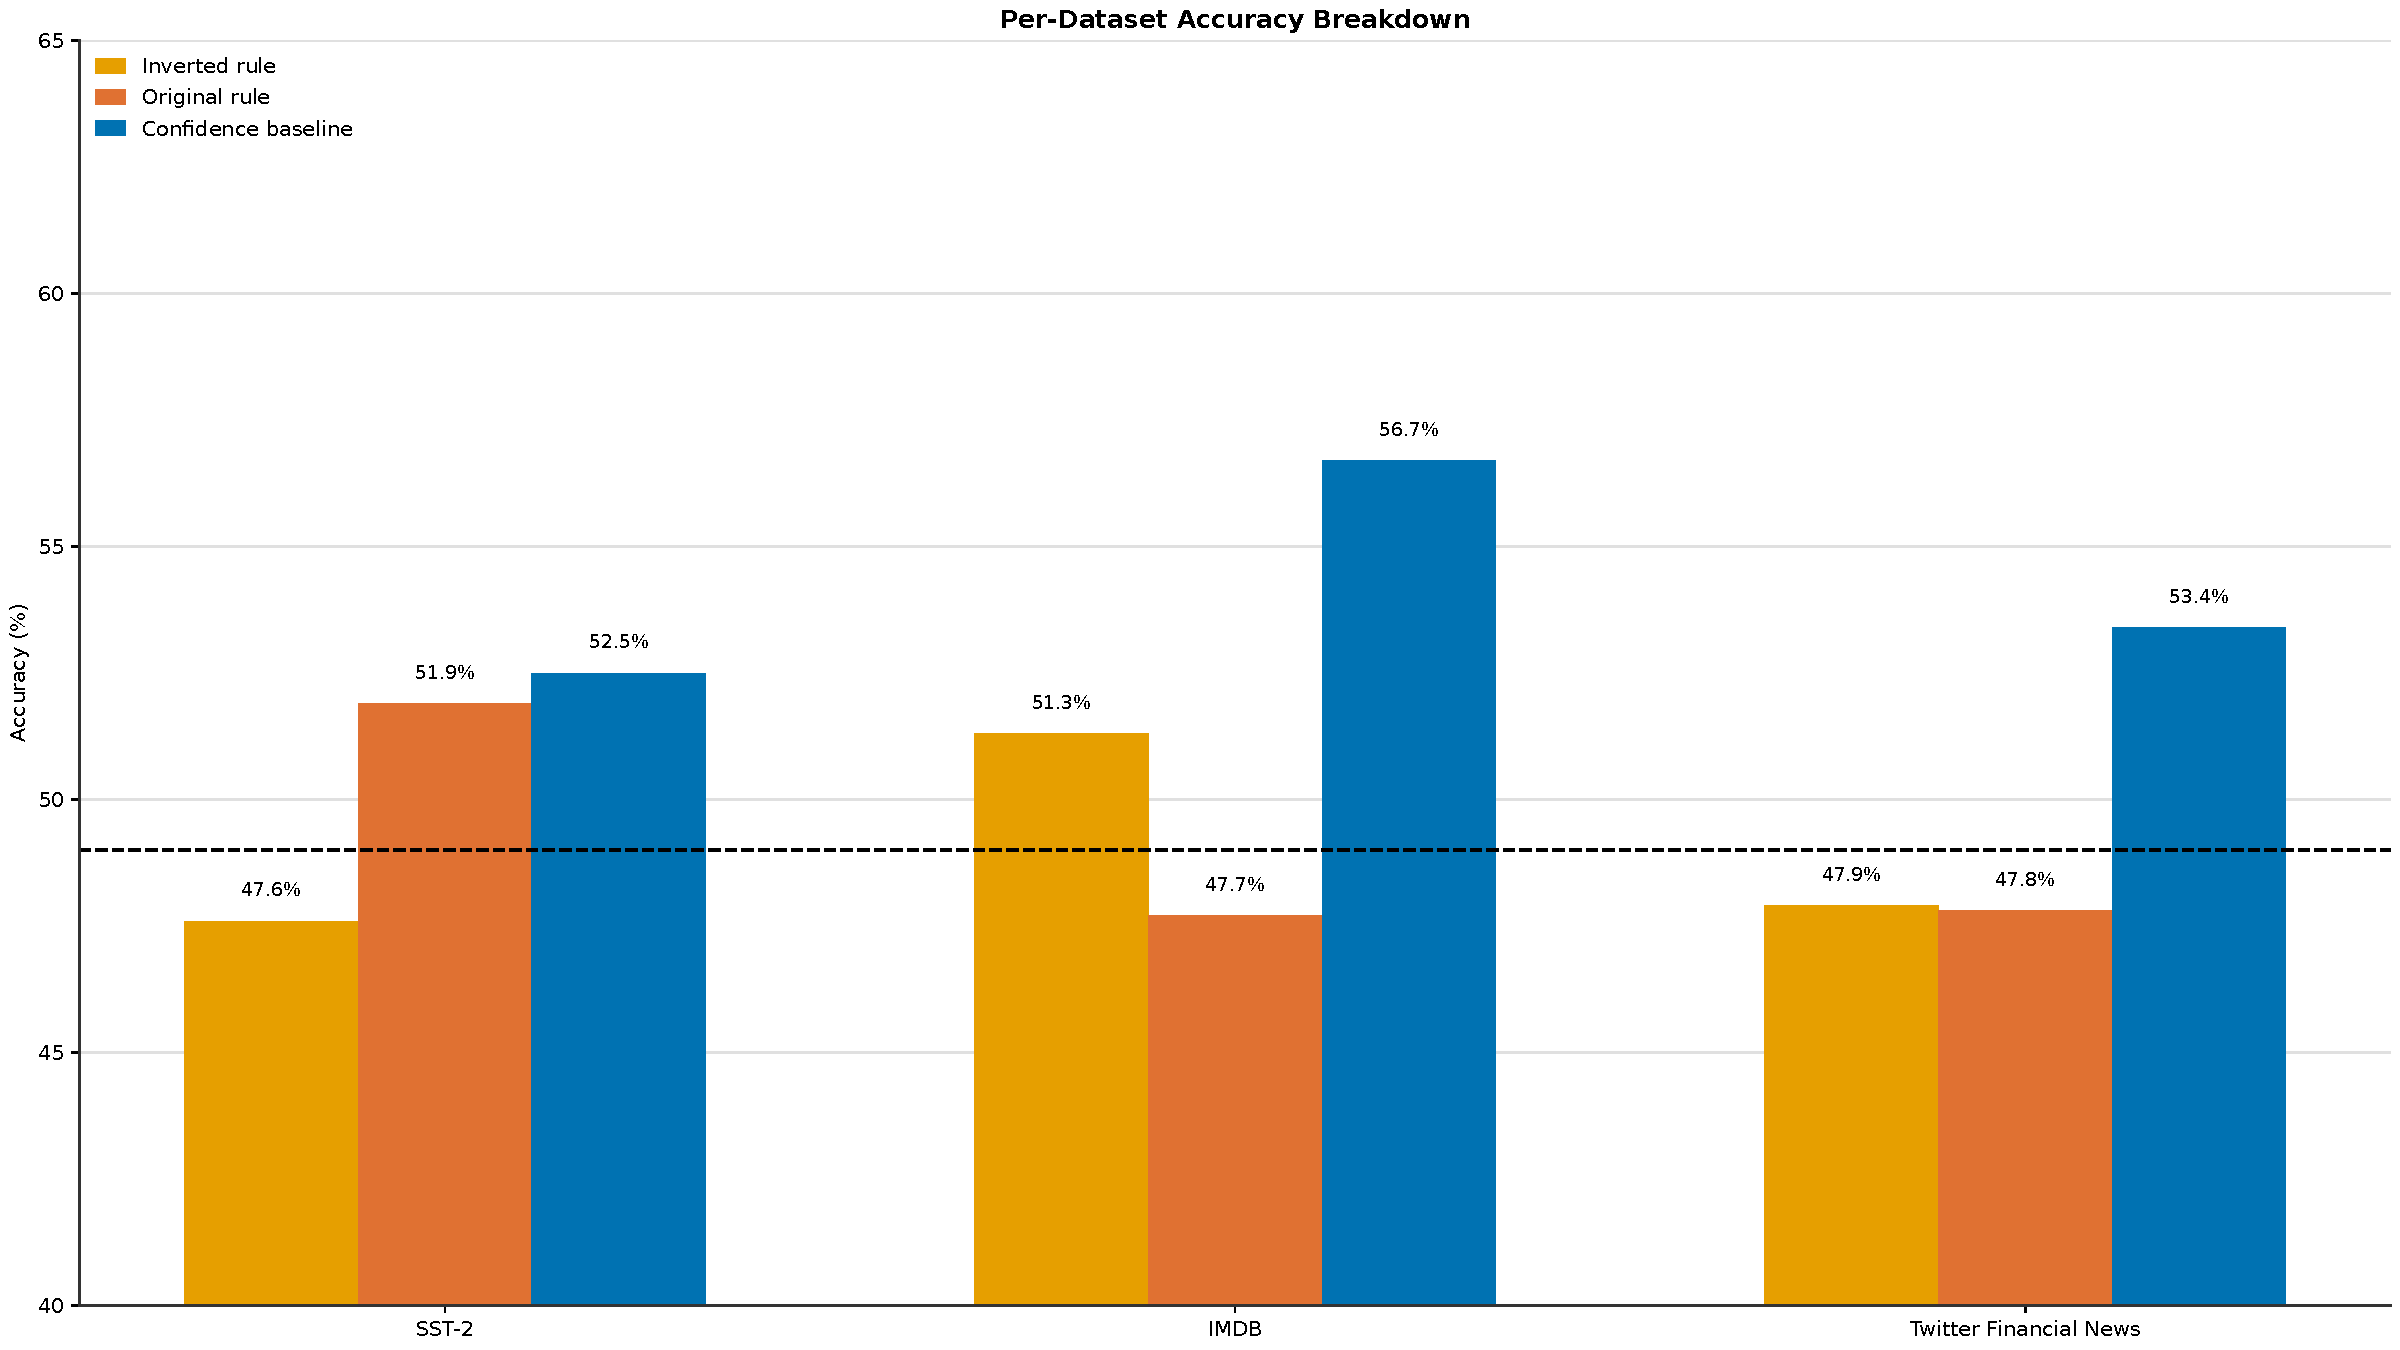
\includegraphics[width=\linewidth,height=0.85\textheight,keepaspectratio]{figures/fig3_v0.pdf}
  \caption{Mean accuracy broken down by dataset. The pattern holds across all three datasets: both directional rules perform at chance while the confidence baseline exceeds chance. IMDB shows the largest confidence gap (56.7\% vs 49.0\%).}
  \label{fig:fig3}
\end{figure}

The pattern holds across all three datasets. On IMDB, the confidence baseline achieves the highest accuracy (56.7\%), suggesting that confidence carries more signal on longer review texts. On SST-2 and Twitter Financial News, the confidence baseline is lower (52.5\% and 53.4\%), but still above both directional rules.

\subsection{Per-Model-Pair Breakdown}

The results are consistent across both model pairs. For logistic regression vs. random forest, the inverted rule achieves 50.7\% and the original rule achieves 46.7\%. For Naive Bayes vs. SVM, the inverted rule achieves 47.3\% and the original rule achieves 51.3\%. Neither pair shows a systematic directional signal.

\subsection{Effect of Sample Size and Imbalance}

The inverted rule's accuracy varies from 41.6\% at sample size 100 to 51.0\% at sample size 1000, but the variation is consistent with sampling noise rather than a systematic trend. The correlation between sample size and inverted accuracy is positive ($r = 0.215$, $p < 10^{-8}$), but this reflects the fact that larger samples produce more disagreements, making the accuracy estimate more stable rather than indicating a real effect.

The accuracy varies across imbalance ratios: 47.3\% at ratio 1.0, 52.2\% at ratio 1.5, and 47.4\% at ratio 2.0. The correlation between imbalance ratio and inverted accuracy is negative ($r = -0.133$, $p = 0.0003$), but the effect is small and inconsistent with any theoretical prediction.

\subsection{Statistical Significance}

Of 652 configurations with disagreements, 67 (10.3\%) show raw significance at $p < 0.05$. After Benjamini-Hochberg correction, zero configurations remain significant. The mean raw p-value is 0.616, and the mean adjusted p-value is 1.0.

\subsection{Feature Confound Analysis}

Our previous study reported 42.4\% accuracy for the original directional rule \footnote{Code: \url{https://github.com/ai-inventor-papers/ai-invention-2f324c-disagreement-asymmetry-oracle/tree/main/round-1/experiment-1}}. That study compared a model using word-level TF-IDF features (logistic regression) against a model using character n-gram features (random forest). The 42.4\% result --- 7.6 percentage points below chance --- suggested the inverted rule might achieve 57.6\%.

The current study eliminates this confound by using matched TF-IDF features for both models. With matched features, the original rule achieves 49.0\% and the inverted rule achieves 49.0\%. The 42.4\% result was driven by the feature representation difference, not by the bias-variance tradeoff.

\begin{figure}[!htbp]
  \centering
  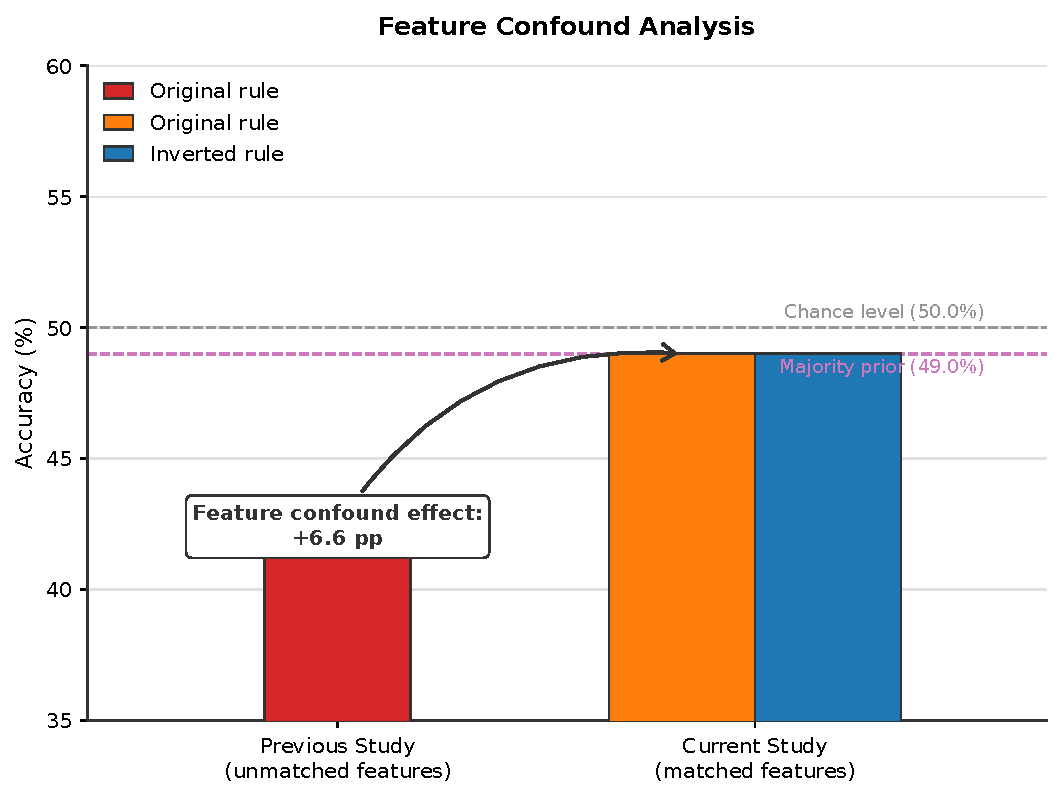
\includegraphics[width=\linewidth,height=0.85\textheight,keepaspectratio]{figures/fig4_v0.pdf}
  \caption{Comparison of the original directional rule accuracy between the previous study (unmatched features: word-level TF-IDF vs. character n-grams) and the current study (matched features: both use TF-IDF word n-grams). The 42.4\% result from the previous study was driven by the feature confound and disappears when both models share features.}
  \label{fig:fig4}
\end{figure}

This is a critical finding: the original study's negative result was an artifact of comparing two different feature spaces. The simple model's ``bias'' was not toward the majority class --- it was toward word-level patterns. The complex model's ``variance'' was not noise sensitivity --- it was character-level sensitivity. Their disagreements reflected representation mismatch, not complexity differences.

\section{Discussion}

\subsection{Why the Hypothesis Failed}

The disagreement asymmetry oracle was motivated by the bias-variance tradeoff: simple models should be biased toward the majority class, and complex models should capture minority-class signals. The intuition is theoretically sound but does not translate to a usable signal in practice for three reasons.

\textbf{First}, the bias-variance tradeoff operates at the population level, not the instance level. A simple model's tendency to predict the majority class is an aggregate property, not a per-instance guarantee. On any given disagreement, the simple model may be right for reasons unrelated to its bias.

\textbf{Second}, even with matched features, the two models in each pair have different inductive biases that do not align with the majority-minority axis. Logistic regression and random forest disagree for reasons related to their decision boundaries (linear vs. tree-based), not to their treatment of class balance. Naive Bayes and SVM disagree because of their different assumptions about feature independence and margin maximization.

\textbf{Third}, the sentiment classification task may not exhibit the kind of noise structure that the hypothesis requires. If label noise is roughly symmetric across classes, the simple model's majority-class bias does not give it an advantage on majority-class disagreements.

\subsection{What the Negative Result Means}

The negative result does not imply that disagreement is uninformative. The confidence baseline achieves 54.3\% accuracy, above chance, showing that the \textit{magnitude} of disagreement (as captured by calibrated confidence scores) does carry signal. The oracle baseline achieves 67.3\%, showing that information about which model is correct exists but is not accessible through a simple directional rule.

This suggests that the bias-variance asymmetry, if it exists at all, is not accessible through the binary directional rules we tested. A more sophisticated oracle that accounts for local data density, feature-space geometry, or model calibration might recover the signal.

\subsection{Limitations}

Our study has several limitations. We test two model pairs on three sentiment datasets. The hypothesis might hold for other model families (e.g., neural networks vs. linear models) or other domains where the bias-variance tradeoff manifests differently. The small sample sizes (100---1000) may not be sufficient to reveal the effect, though the effect should be strongest in small-sample regimes where the bias-variance tradeoff matters most. We do not test the effect of model calibration on the directional rule itself, only on the confidence baseline.

\subsection{Multi-Model Extension}

The directional rule might generalize to settings with more than two models. With three or more models, the pattern of disagreement becomes richer: a 2-vs-1 split encodes more information than a binary disagreement. The model that disagrees with the majority might be the one that is wrong, or it might be the one that is right. This question remains open.

\section{Conclusion}

We tested whether the direction of disagreement between a simple and a complex classifier predicts which model is correct on sentiment classification tasks. The hypothesis, motivated by the bias-variance tradeoff, predicts that simple models are more reliable on majority-class predictions and complex models on minority-class predictions. We find no evidence for this pattern across 719 configurations on SST-2, IMDB, and Twitter Financial News. Both the original and inverted directional rules achieve 49.0\% accuracy, indistinguishable from the majority-class prior. The original 42.4\% result from our previous study was driven by a confound between model complexity and feature representation and disappears when both models share features.

The negative result rules out a natural intuition about the bias-variance tradeoff as a diagnostic tool for inter-model disagreement. Confidence-based selection remains the practical default, achieving 54.3\% accuracy on disagreement samples.

\noindent\textbf{Future work}:
\begin{itemize}
  \item Test the hypothesis on image classification and tabular datasets.
  \item Investigate whether neural network model pairs exhibit directional asymmetry.
  \item Study whether multi-model disagreement patterns (e.g., 2-vs-1 splits) carry more signal than binary disagreements.
  \item Develop oracles that combine directional information with local data density or feature-space geometry.
\end{itemize}

\bibliography{references}
\bibliographystyle{plainnat}

\end{document}
